%++++++++++++++++++++++++++++++++++++++++
% Don't modify this section unless you know what you're doing!
\documentclass[letterpaper,12pt]{article}
\usepackage{tabularx} % extra features for tabular environment
\usepackage{amsmath}  % improve math presentation
\usepackage{mathabx}
\usepackage{braket}
\usepackage{siunitx}
\usepackage{graphicx} % takes care of graphic including machinery
\usepackage[margin=1in,letterpaper]{geometry} % decreases margins
\usepackage{cite} % takes care of citations
\usepackage[final]{hyperref} % adds hyper links inside the generated pdf file
\usepackage{blkarray}
\usepackage{multirow}
\usepackage{tikz}
\usetikzlibrary{calc}
\hypersetup{
	colorlinks=true,       % false: boxed links; true: colored links
	linkcolor=blue,        % color of internal links
	citecolor=blue,        % color of links to bibliography
	filecolor=magenta,     % color of file links
	urlcolor=blue         
}
%++++++++++++++++++++++++++++++++++++++++


\begin{document}

\title{Report IV}
\author{Cristina Mier Gonz\'alez}
\date{\today}
\maketitle

\begin{abstract}
In this report I explain the deduction of the Rashba Hamiltonian caused by the spin-orbit-coupling and how to add this interaction to the atomic chain program. I performed simulations for a dimer of Cr atoms in $\beta$-Bi$_2$Pd and observed the dependency of the in-gap states with the distance between sites. Also, I studied system of long atomic chains where I search for edge states at zero energy.

%Explain Rashba Hamiltonian, write explicit matrix. Some results in dimer and atomic chain.
\end{abstract}

\section{Spin-orbit coupling: Rashba Hamiltonian}
For a flat surface, with an electric field perpendicular to the $xy$ plane, the Rashba Hamiltonian is written \cite{Manchon2015}:
\begin{equation}
    \hat{H}_{Rashba} = \frac{\alpha_R}{\hbar}(\Vec{\sigma}\times\Vec{p})_z
\end{equation}
Where $\alpha_R$ is the spin-orbit coupling strength and $\Vec{\sigma} = (\sigma_x, \sigma_y, \sigma_z)$ are the spin Pauli matrices. In a 2D system, where electrons are confined in the $xy$ plane, the Rashba Hamiltomian becomes:
\begin{equation}
    \hat{H}_{Rashba} = \frac{\alpha_R}{\hbar}(p_y\sigma_x - p_x\sigma_y)
    \label{2D}
\end{equation}
The momentum operator is related to the differential operator:
\begin{equation}
    \hat{p}_x = -i\hbar\frac{\partial}{\partial x} \qquad \hat{p}_y = -i\hbar\frac{\partial}{\partial y}
\end{equation}
Using finite differences and the following discretization of the 2D space as $\ket{n, m} = \ket{x = na, y = ma}$ states where $a$ is the lattice parameter, the momentum operators become\cite{thesis}:
\begin{equation}
    \hat{p}_x = -i\hbar \frac{\ket{n+1, m}\bra{n, m}}{2a} \qquad  \hat{p}_y = -i\hbar \frac{\ket{n, m+1}\bra{n, m}}{2a}
\end{equation}
The Rashba Hamiltonian is now writen:
\begin{equation}
    \hat{H}_{Rashba} = \frac{\alpha_R}{2a}\sum_{n, m, \sigma}\Bigg[ \big(\ket{n+1, m}_\sigma\bra{n, m}_{\sigma'}\times i\sigma_y\big) - \big(\ket{n, m+1}_{\sigma}\bra{n, m}_{\sigma'}\times i\sigma_x \big)\Bigg] + h.c.
     \label{tight}
\end{equation}
The subindex $\sigma$ indicates the spin of each state. The Hamiltonian couples states at nearest neighbours sites and with different spin state. \\ \\
%We want to write Equation \ref{tight} in matrix form using the Nambu basis $\Psi = [\psi_\uparrow \psi_\downarrow \psi_\uparrow^\dagger \psi_\downarrow^\dagger]^T$. For the coupling along the $x$ direction we have:
$\sigma_x$ and $\sigma_y$ are two-dimension matrices covering the two spin states $\uparrow$ and $\downarrow$. 
However, we want to write equation \ref{tight} using the four-component Nambu basis: $\Psi = [\psi_\uparrow \psi_\downarrow \psi_\uparrow^\dagger \psi_\downarrow^\dagger]^T$, where the two last components correspond to the time-reversed states. Like this, the Rashba Hamiltonian in this four component space becomes:\\ \\ 
\vspace{.5cm}
\begin{equation}
\footnotesize
\hat{H}_{Rashba} = \frac{\alpha_R}{2a}
    \begin{pmatrix}
    0 & \hat{p}_x - i\hat{p}_y\quad\hat{p}_x^\dagger + i\hat{p}_y^\dagger & 0 & 0\\
    -\hat{p}_x + i\hat{p}_y\quad-\hat{p}_x^\dagger - i\hat{p}_y^\dagger & 0 & 0 & 0\\
    0 & 0 & 0 & -\hat{p}_x + i\hat{p}_y\quad-\hat{p}_x^\dagger - i\hat{p}_y^\dagger\\
    0 & 0 & \hat{p}_x - i\hat{p}_y\quad\hat{p}_x^\dagger + i\hat{p}_y^\dagger & 0
    \end{pmatrix}
\end{equation}
\vspace{.5cm}

Where the upper block correspond to the electron space and the lower block is the time-reversed or hole space. The timer reversed Hamiltonian is obtained by taking the minus complex conjugate, this is, $ - \hat{H}^\dagger$. Nevertheless, when writing this matrix for the superconducting array of dimension $N_x \times N_y$, I need to differentiate between the Rashba coupling in the $x$ and $y$ direction.\\ \\
To understand this issue, I will explicitly write the matrix of the Rashba interaction, for the case where $N_x = 2$ and $N_y = 3$. The corresponding latticed is depicted in Figure \ref{diagram}, where each node is labelled with the corresponding state $\ket{n, m}$.\\ \\
\begin{figure}[h!]
\centering
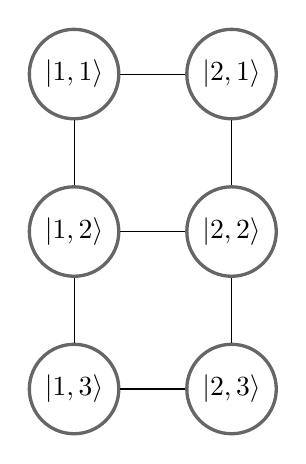
\begin{tikzpicture}[node distance=2cm, roundnode/.style={circle, draw=black!60, very thick, minimum size=7mm},]  
\node[roundnode](1)                      {$\ket{1,1}$};
\node[roundnode](2)         [right of=1]{$\ket{2,1}$};
\node[roundnode](3)         [below of=1]{$\ket{1,2}$};
\node[roundnode](4)                      [below of=2]{$\ket{2,2}$};
\node[roundnode](5)                      [below of=3]{$\ket{1,3}$};
\node[roundnode](6)                      [below of=4]{$\ket{2,3}$};

\draw(1) -- (2);
\draw(1) -- (3);
\draw(2) -- (4);
\draw(3) -- (4);
\draw(1) -- (3);
\draw(3) -- (5);
\draw(4) -- (6);
\draw(5) -- (6);

\end{tikzpicture} 
\label{diagram}
\caption{Lattice with $N_x = 2$ and $N_y = 3$ resulting in 6 sites lattice, labelled using the notation $\ket{n, m}$.}
\end{figure}
\clearpage
The resulting matrix will have total size $24 \times 24$, because the lattice has 6 sites times the 4 Nambu components. Explicitly:
\[
\renewcommand\arraystretch{1.75}
%\footnotesize
\begin{blockarray}{rccccccccc}
&&& \ket{1, 1} & \ket{2, 1} & \ket{1, 2} & \ket{2, 2} & \ket{1, 3} & \ket{2, 3} &\\
\begin{block}{rc[c@{}c|c|c|c|c|c@{}c]}
  & \bra{1, 1} &&  & \hat{H}_x & \hat{H}_y &  &  & &\vphantom{\smash[b]{\bigg|}} \\
\BAhhline{~~~------~}
  & \bra{2,1} && \hat{H}_x^\dagger &  & & \hat{H}_y  &  & &\\
\BAhhline{~~~------~}
\hat{H}_{Rashba}=\quad
 & \bra{1,2} &&  \hat{H}_y^\dagger  &  &  &  \hat{H}_x &  \hat{H}_y  & &\\
\BAhhline{~~~------~}
  & \bra{2,2} &&  &  \hat{H}_y^\dagger  &  \hat{H}_x^\dagger  &  &   & \hat{H}_y \\
\BAhhline{~~~------~}
 & \bra{1,3} &&  &  &  \hat{H}_y^\dagger &  &  &  \hat{H}_x &\\
 \BAhhline{~~~------~}
  & \bra{2,3} &&  &  &  & \hat{H}_y^\dagger & \hat{H}_x^\dagger  & \vphantom{\smash[t]{\bigg|}} &\\
\end{block}
\end{blockarray}
\]
Each of the sites of the previous matrix has actually size $4\times 4$. As we can see, the Rashba Hamiltonian has been divided between $x$ and $y$ coupling. Note that the diagonal blocks are empty and given the state $\ket{n,m}$ only the sites where $n$ ($m$) differs in a unit have Rashba coupling along $x$ ($y$) direction.
The $\hat{H}_x$ and $\hat{H}_y$ are given:
\vspace{0.5cm}
\begin{equation}
\hat{H}_x = 
    \frac{\alpha_R}{2a}\begin{pmatrix}
    0 & 1 & 0 & 0 \\
    -1 & 0 & 0 & 0 \\
    0 & 0 & 0 & -1 \\
    0 & 0 & 1 & 0
  \end{pmatrix}
\end{equation}
\vspace{0.5cm}
\begin{equation}
\hat{H}_y = 
    \frac{\alpha_R}{2a}\begin{pmatrix}
    0 & -i & 0 & 0 \\
    -i & 0 & 0 & 0 \\
    0 & 0 & 0 & -i \\
    0 & 0 & -i & 0
  \end{pmatrix}
\end{equation}

\vspace{0.5cm}
The Rashba Hamiltonian is added to the Self energy matrix, $\Sigma$, as a perturbation to the BCS Hamiltonian. The Green's function of the total system which allows us to obtain the spectrum is obtained by solving Dyson's equation:
\begin{equation}
    G = [1 - G_o\Sigma]^{-1}G_o
\end{equation}

\section{Results}
Using the program introduced in previous reports, the chain of adatoms on the supercondcuting matrix, I performed several simulations for different chain lengths. Here I summarize the most interesting results for the dimer and the long atomic chains.
\subsection{Dimer}
The dimer results were already summarize in Report I. However, improvements in the representation allows for a better visualization of the effect of the potential scattering as well as the effect of the SOC.\\ \\
In the case of a dimer, the size of the superconductor underneath the magnetic atoms, has not a big effect on the resulting spectrum. Like this, the simulations are performed taking a lattice of size $N_x = 4$ and $N_y = 3$.\\ \\
\begin{figure}[h!]
    \centering
    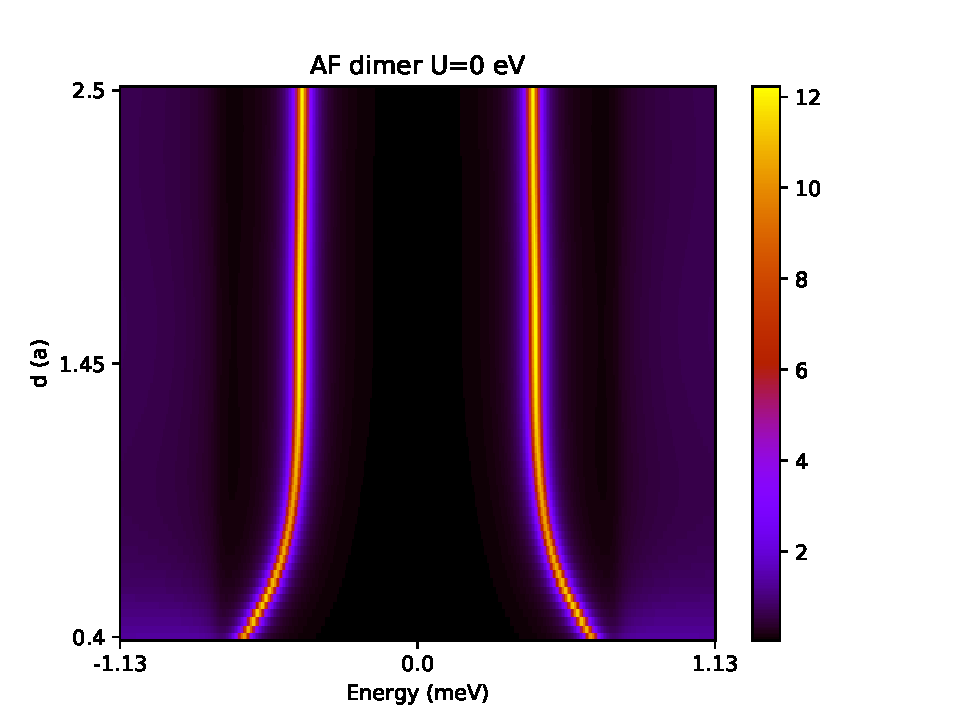
\includegraphics[scale = .5]{AF_dimer.pdf}
    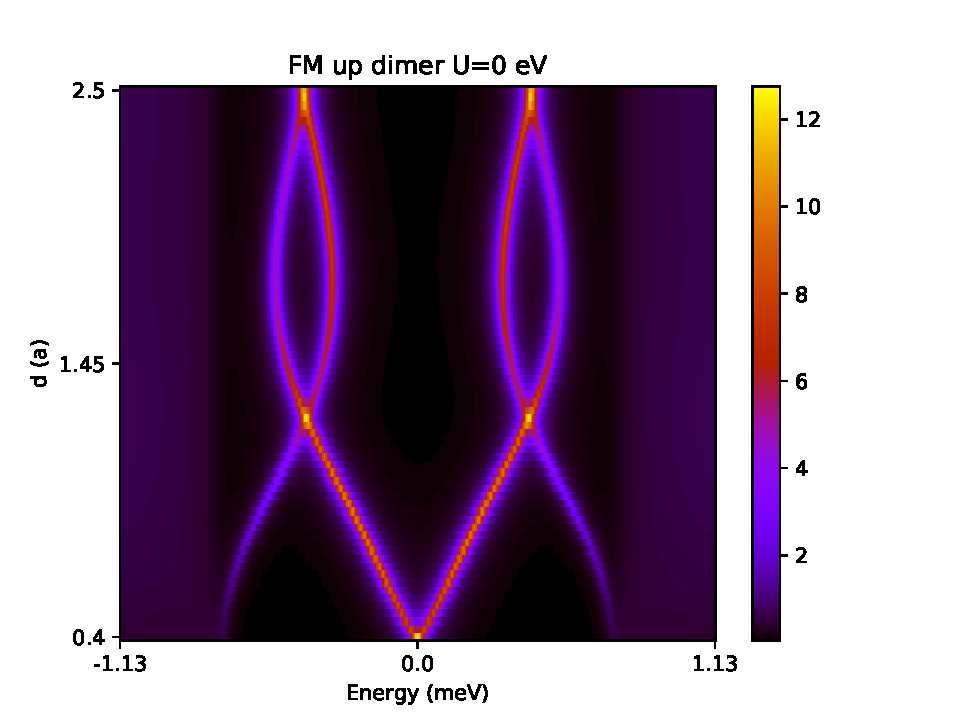
\includegraphics[scale = .5]{FM_dimer.pdf}
    
    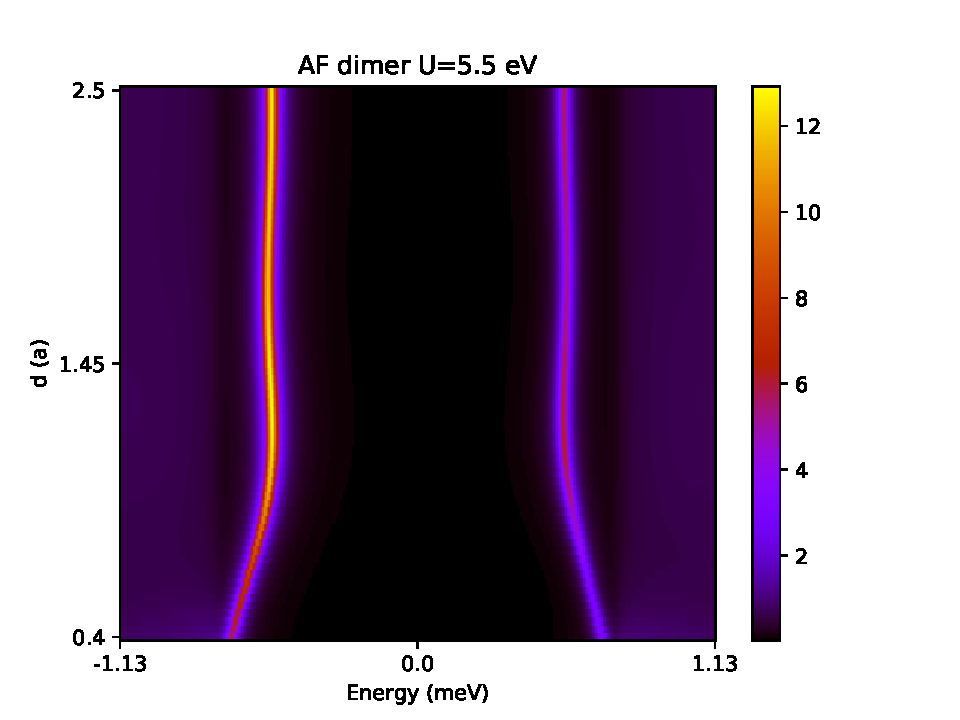
\includegraphics[scale = .5]{AF_dimer_U5_5.pdf}
    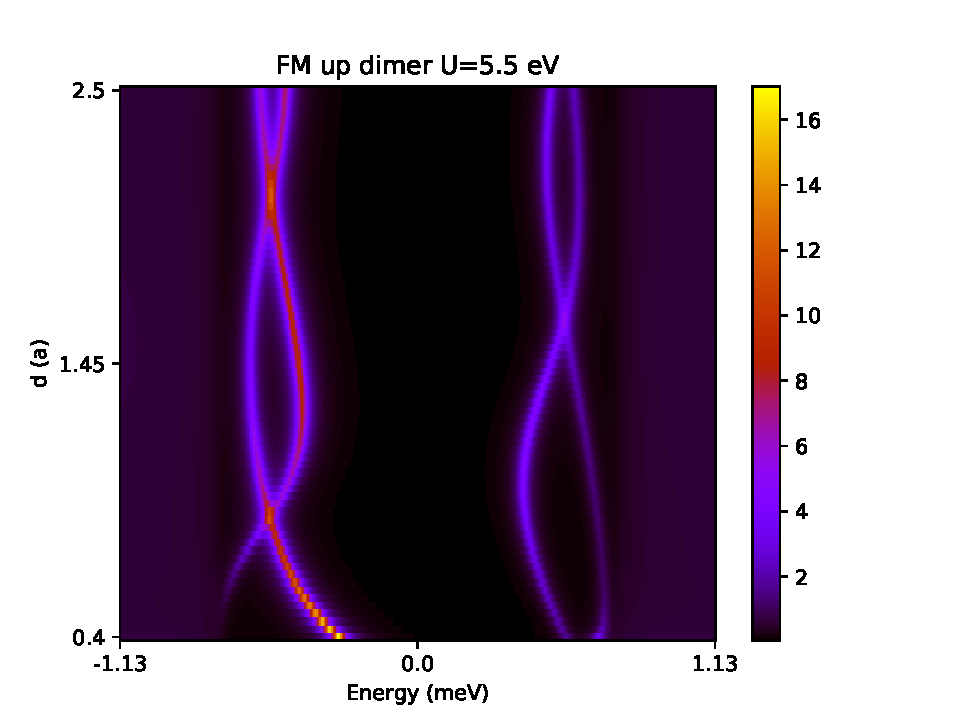
\includegraphics[scale = .5]{FM_dimer_U5_5.pdf}
    
    \caption{2D maps of distance between lattice sites versus energy spectrum with no SOC, the PDOS of the states is represented as a heat map.}
    \label{dimernoSOC}
\end{figure}

I want to observe the different spectra for a varying distance between sites in the lattice, more specifically, the position of the Shiba peaks appearing inside the superconducting gap. For this I performed several simulations varying the distance $d = na$, where $a$ is the lattice parameter of the superconductor. The parameters used in the simulations are the following: $k_F = 0.4$ a.u., $\Delta = 0.75$ meV, $J=1.8$ eV, the spin of the magnetic atoms is 5/2 (Cr), the potential scattering is taken as zero and $U = 5.5$ eV and the SOC is zero.\\ \\
The results are shown in Figure \ref{dimernoSOC}, where I plotted the distance between sites versus the energy of the Shiba states, the height of the peaks is represented as a heat map. In the two upper panels I shown the results for the case without potential scattering for the spin states anti-ferromagnetic (AF) $\uparrow\downarrow$ and ferromagnetic (FM) $\uparrow\uparrow$. The AF state shows two clear peaks with symmetric position and height. For smaller distances these two states start to shift toward higher energies. On the other hand, the FM state shows four in-gap states with an oscillatory behaviour resulting in the crossing of the states, the value $k_F = 0.4$ is chosen so we can observe these oscillations. In the two lower panels we observe the same results but with a potential scattering of $U = 5.5$ eV, for AF state we observe similar results, however, althought the in-gap are still symmetric in energy the height is not the same. In the FM case, the Shiba states still shown an oscillatory behaviour, however the symmetry in both height and position is broken. These results are in good agreement with what is shown in the supplementary material in reference\cite{DJ}.\\ \\ 
\begin{figure}[h!]
    \centering
    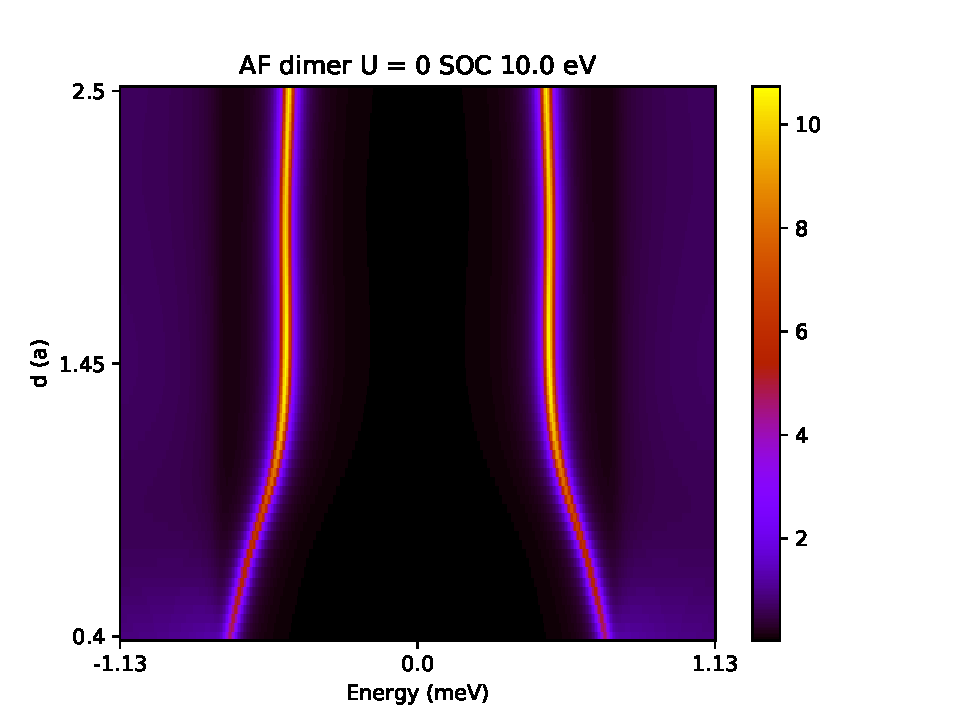
\includegraphics[scale = .5]{AF_dimer_SOC_10.pdf}
    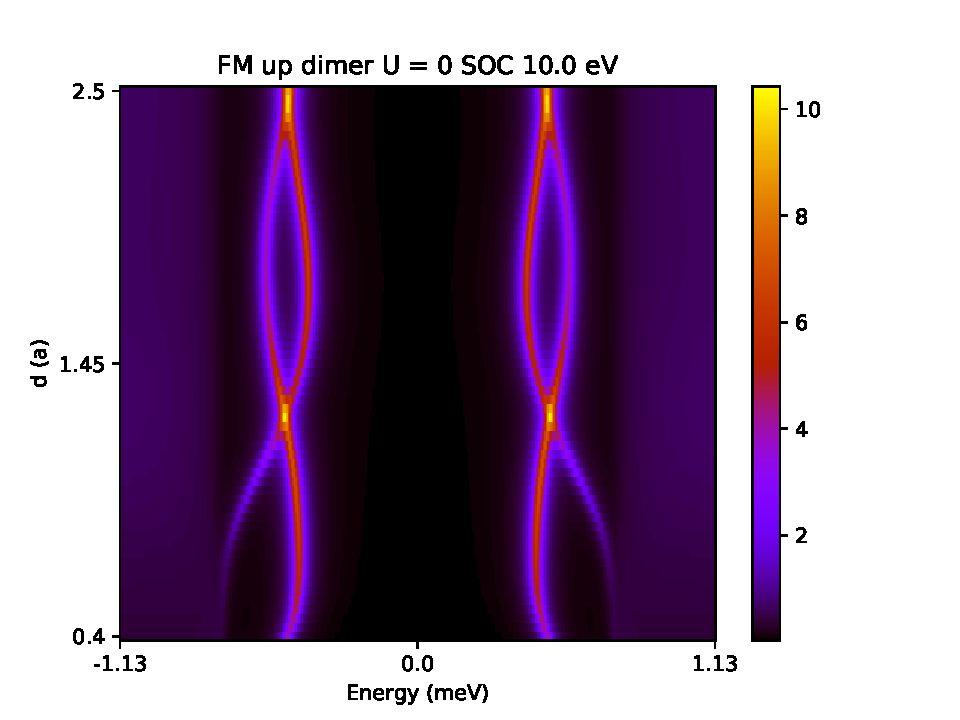
\includegraphics[scale = .5]{FM_dimer_SOC_10.pdf}
    
    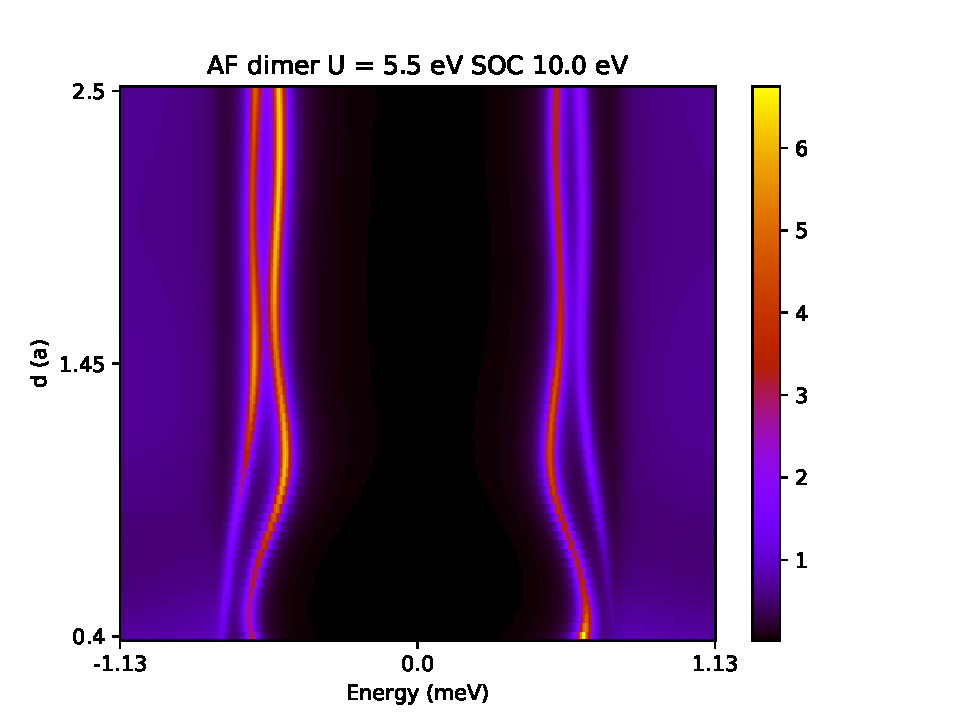
\includegraphics[scale = .5]{AF_dimer_SOC_10_U.pdf}
    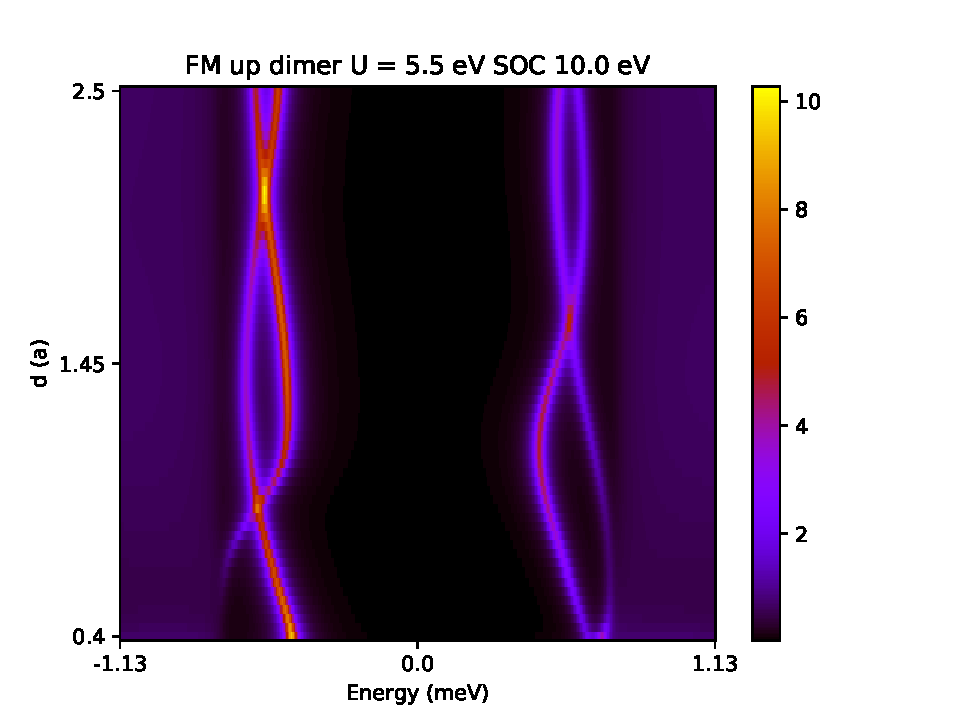
\includegraphics[scale = .5]{FM_dimer_SOC_10_U.pdf}
    
    \caption{2D maps of distance between lattice sites versus energy spectrum, the PDOS is represented in the $z$ direction as a heat map with $\alpha_R = 10.0$ eV$\cdot$A.}
    \label{dimerwithSOC}
\end{figure}

Next, I performed the same study including the spin-orbit interaction. On Figure \ref{dimerwithSOC} we can see the results for a SOC strength of $\alpha_R =10.0$ eV$\cdot$A. When compared to the previous plots without SOC, we observe very similar behaviour. However, for all spectrum, we can see that the Shiba states have shifted to higher energies. Also if we look at the AF states with potential scattering we can see that in the presence of SOC, the two peaks have split into four. I took a $\alpha_R$ unrealistically high to better appreciate the influence of the SOC, however for results with $\alpha_R = 4.5$ eV$\cdot$A, the same effect can also be appreciated.

 
\subsection{Atomic chains}
In this next section, I made some studies of long magnetic chains of adatoms on a superconducting surface. I focused in the search of Majorana edge states which are expected to arise as an in-gap state at zero energy localized towards the ends of the chain. In this study I try to focus on the experimental system of $\beta$-Bi$_2$Pd for the superconducting material and Cr for the magnetic adatoms. I divided the studied in two subsections: in the first one I used the same experimental parameters as in \cite{DJ} setting the potential scattering to zero and in the second one I studied the system including the potential scattering $U = 5.5$ eV.

\subsubsection{Without potential scattering}

In this first study, I simulated long atomic chains situated on top of the superconducting array. As we have seen in the previous section, in the absence of potential scattering, we expect to obtain symmetric spectrum.\\ \\
The atoms are set in FM state with spins pointing up. The chosen parameters are the following: $k_F = 0.183$ a.u., $\Delta = 0.75$ meV, $J = 1.8$ eV, the SOC strength is $\alpha_R = 2.5$ eV$\cdot$A and the spin of the magnetic atoms is 5/2. In a first simulation I studied the system for a chain with 25 atoms. Energies are taken between $\pm 2\Delta$ at 2001 points. The chain is situated in the middle of an array with dimension $N_y = 9$ and $N_x = 33$ sites, meaning that there four empty sites at both ends of the chain and also in the perpendicular direction. The results are depicted in Figure \ref{25Atoms}.\\ \\ 
The upper left panel shows the spectrum in the first atom of the chain, as we can see, it presents a high peak at zero energy with smaller peaks on the sides, from the rest of figures we can conclude that the state is well localized at the ends of the chain. The upper right plot shows the index along the chain versus the spectrum, the PDOS of the states is shown as a heat map, from this plot we can see a state at zero energy with a high density of states in the first and last atom, this is also visible in the lower left plot showing the profile along the chain, the atoms are situated between sites 4 and 29 and we can see an exponential decay of the PDOS reaching zero in the middel of the chain. Finally, I also plotted the projected density of states everywhere in the lattice as shown in the lower panel in the right. From this we can see that the PDOS decays along the chain but also in the perpendicular direction. Similar results are obtained for chains of 30, 40 and 50 atoms, with the prominent peak staying at zero energy and the state well localized. This is still true for atomic lenghts of 20 atoms, below this value, the peak at zero energy splits into two peaks.\\ \\
\begin{figure}[h!]
    \centering
    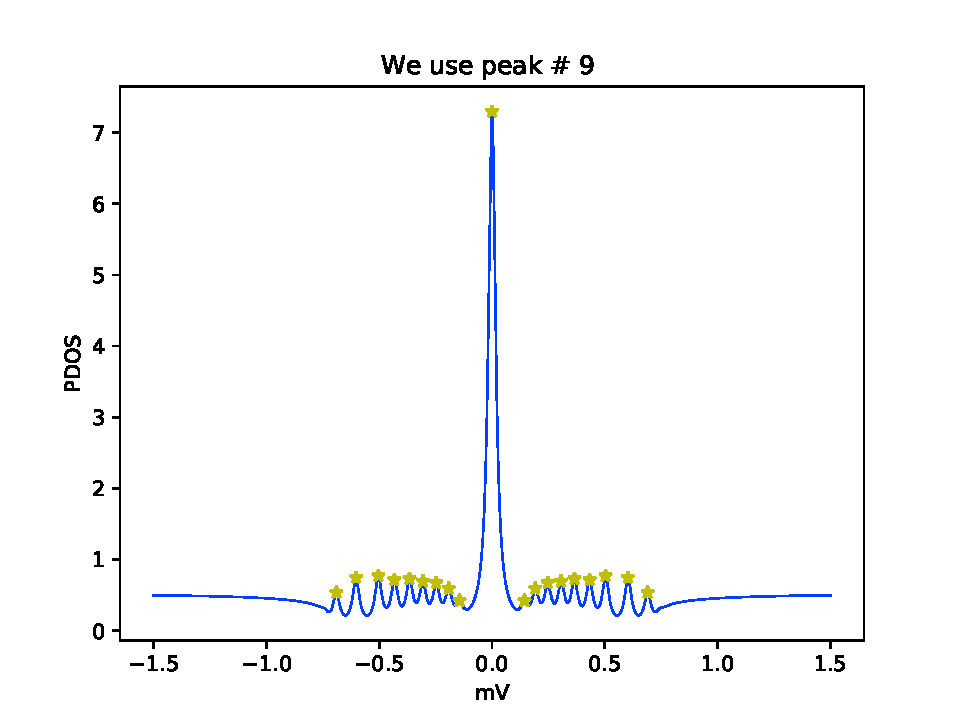
\includegraphics[scale = .5]{spectro.pdf}
    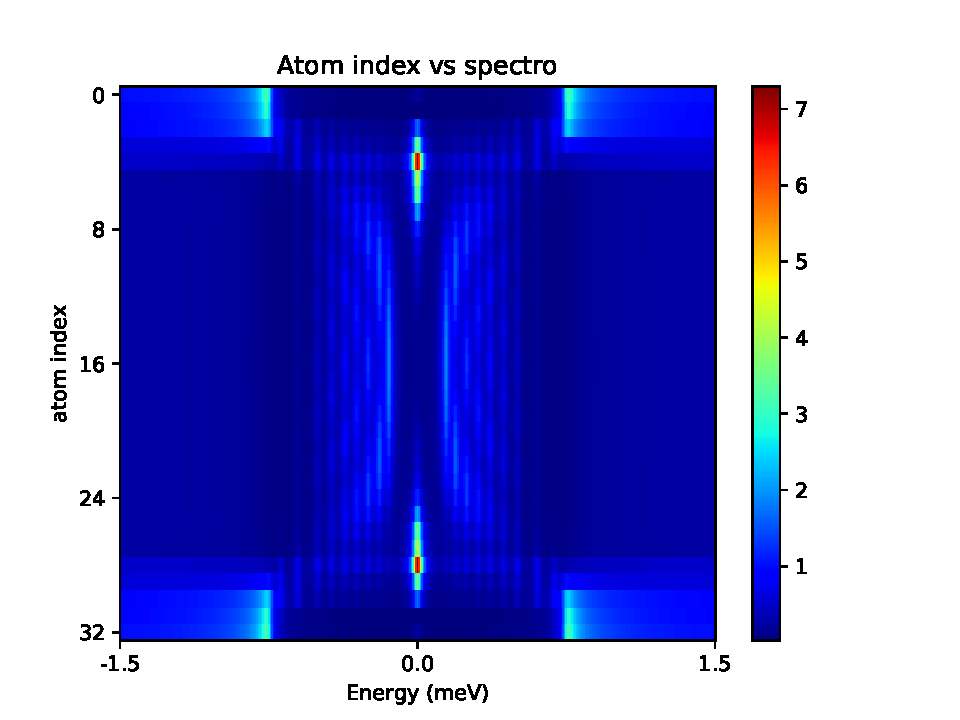
\includegraphics[scale = .5]{map.pdf}
    
    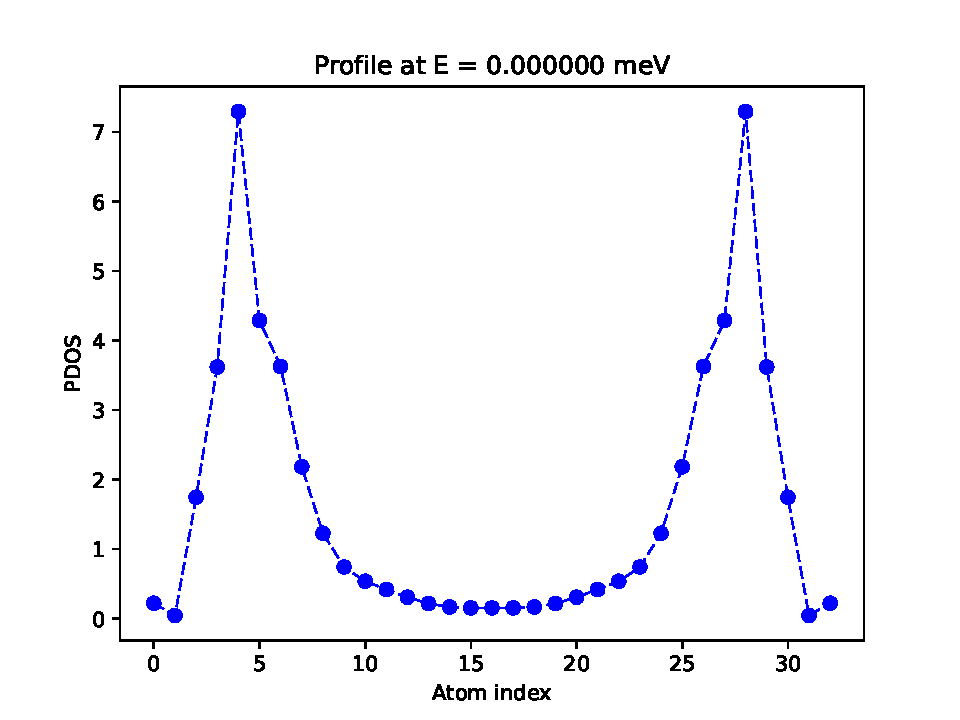
\includegraphics[scale = .5]{profile.pdf}
    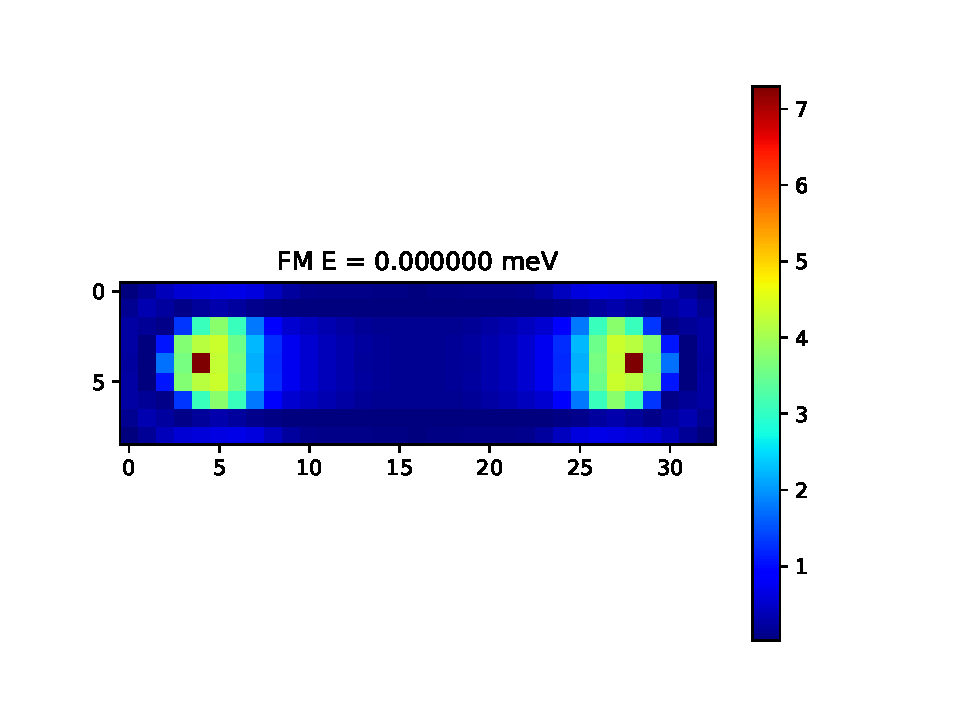
\includegraphics[scale = .5]{2D.pdf}
    
    \caption{Results for Cr chain with 25 atoms on $\beta$-Bi$_2$Pd without potential scattering. \textit{Top left}: Spectrum in first atom. \textit{Top right}: Atom index along the chain vs spectrum. \textit{Bottom left}: 2D map of the PDOS in the complete array. \textit{Bottom right}: Profile of PDOS for $E = 0.0$ eV along the the atomic chain.}
    \label{25Atoms}
\end{figure}


\subsubsection{With potential scattering}

In order to make the simulation more realistic, in this last study I keep on searching localized states at zero energy, but adding the potential scattering. As we saw for the dimer, this parameter induces disorder and results in asymmetric spectrum.\\ \\
I first made a simulation taking the same parameters as in the previous subsection, but adding $U = 5.5$ eV. However, the resulting spectrum does not show any state as zero energy. I performed more simulations changing $k_F = 0.0412$ and adjusting $\alpha_R$ so I could find a peak close to zero energy. On Figure \ref{22Atoms_U} we can see the results obtained for the following parameters: $k_F = 0.0412$ a.u., $\Delta = 0.75$ meV, $J = 1.8$ eV, the SOC strength is $\alpha_R = 23.2$ eV$\cdot$A. The length of the chain is 22 atoms.\\ \\ 

\begin{figure}[h!]
    \centering
    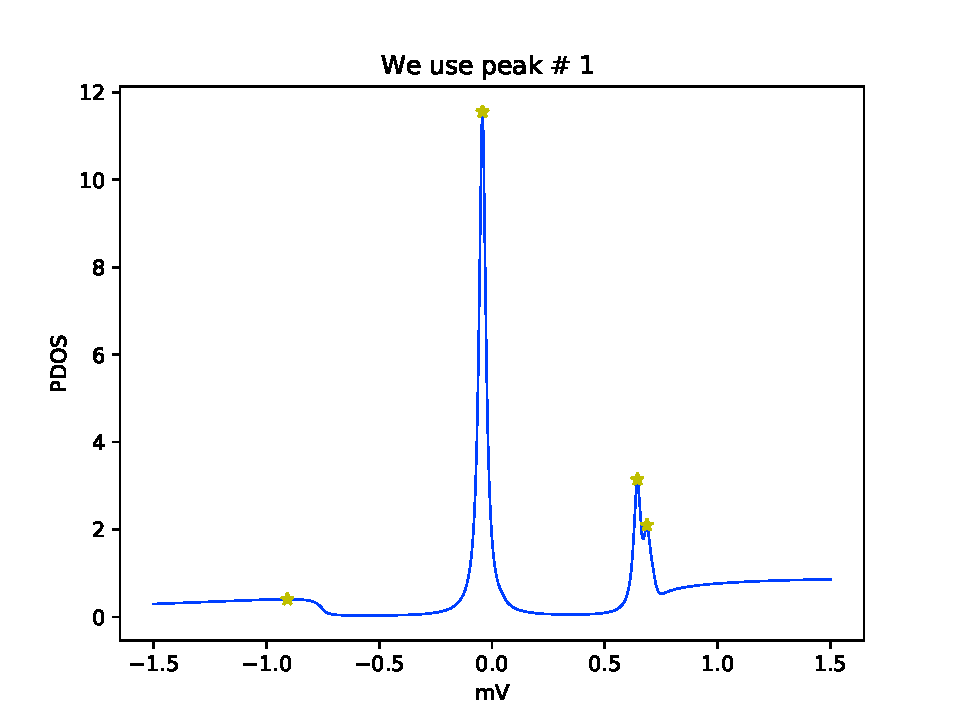
\includegraphics[scale = .5]{spectro_U.pdf}
    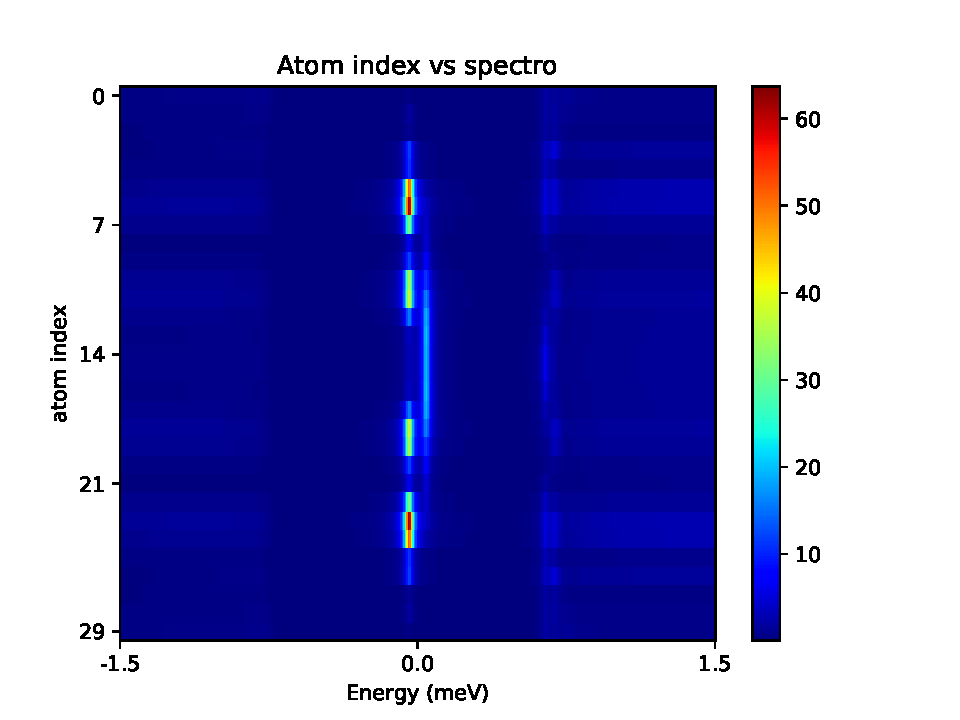
\includegraphics[scale = .5]{map_U.pdf}
    
    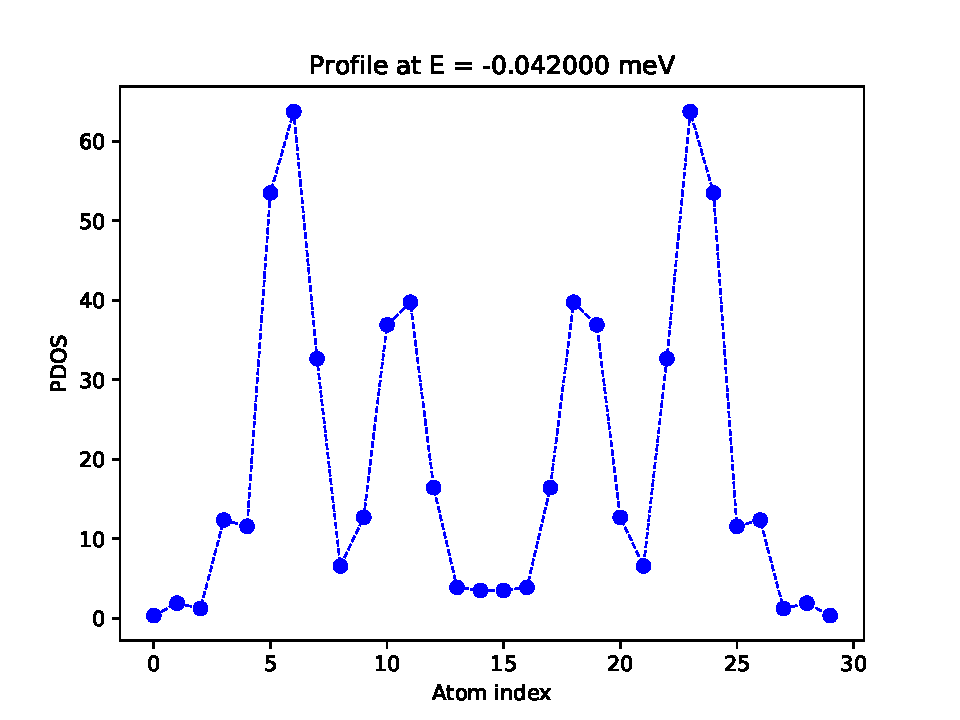
\includegraphics[scale = .5]{profile_U.pdf}
    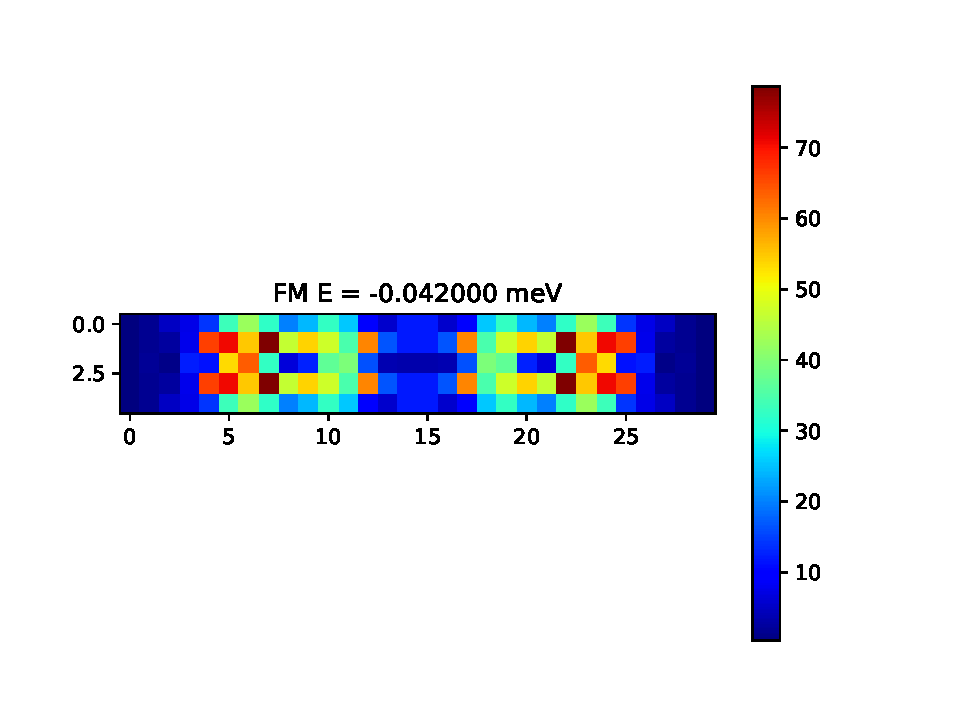
\includegraphics[scale = .5]{2D_U.pdf}
    
    \caption{Results for Cr chain with 22 atoms on $\beta$-Bi$_2$Pd with potential scattering $U = 5.5$ eV. \textit{Top left}: Spectrum in first atom. \textit{Top right}: Atom index along the chain vs spectrum. \textit{Bottom left}: 2D map of the PDOS in the complete array. \textit{Bottom right}: Profile of PDOS for $E = 0.0$ eV along the the atomic chain.}
    \label{22Atoms_U}
\end{figure}

In the upper left panel of Figure \ref{22Atoms_U}, I show the spectrum in the first atom, as we can see there is a peak close to zero ($-0.042$ meV). When we look at the map of the atom index versus the spectrum (upper right) and the PDOS profile along the chain, we see that the state is localized in different sites along the chain, although the highest PDOS is found close to the ends of the chain. However, when we look the map of the complete array (lower right panel) we see that the highest density of states is found outside of the chain and does not go to zero in the border of the array. I performed more simulations with a bigger array but keeping the same parameters, but I found that the peak close to zero shifts away to more negative values an the states are still not zero on the borders of this new array.


\clearpage
\bibliography{name.bib}{}
\bibliographystyle{abbrv}


\end{document}
